\documentclass{article}
\usepackage{float}
\usepackage{multirow}
\usepackage[table,xcdraw]{xcolor}
\usepackage{lscape}
\usepackage{longtable}
\usepackage{graphicx}
\usepackage{times}
\usepackage{amsmath}
\usepackage{fdsymbol}
\usepackage{hyperref}
\usepackage[margin=0.6in]{geometry}
\usepackage{multicol}
\usepackage{listings}
\usepackage{xcolor}

\renewenvironment{abstract}
 {\par\noindent\textbf{\abstractname.}\ \ignorespaces}
 {\par\medskip}

\begin{document}

\title{
Part B - Implementation of Algorithm 1}



\maketitle
\tableofcontents

\newpage

\begin{abstract}
\\In  part b we implement cleartext soft decision tree prediction algorithm; algorithm specified in Akavia et al ECML’2020. 
\end{abstract}


\section{Introduction}
Reference to our \href{https://github.com/assiakhateeb/PPML_lab/tree/main/part\%20B}{\textcolor{blue}{Github repo}}.\\
Part b of the lab is done by dividing the problem into multiple phases, each one we called it pre-processing phase.
\begin{itemize}
\item First pre-procssing is scaling the data.
\item Second pre-procssing is preparing the polynom which is required for Algorithm 1.
\item Third pre-procssing is building a tree with 1-hot encoding labels.
\end{itemize}
We predict on set of samples using Algorithm 1.
Then, we present the main results of Algorithm 1 and compare it to scikit learn results.\\


\section{Preprocessing Phase}
In this section, by using preprocessing, input data is processed to produce an output data that is used in our program.

\subsection{SCALING}
We used the sklearn.preprocessing package which provides several common utility functions and transformer classes to change raw feature vectors into a representation that is more suitable for the downstream estimators.\\
\par
We start by re-scaling each value in the given data set, to a value in range \([-1,1]\) (according to the article) using MinMaxScaler package from sklearn.
The general formula to rescale a range between a of values [a, b] is given as:
\begin{equation}
\begin{split}
x' = a + \frac{(x-min(x))(b-a)}{max(x)-min(x)} 
\end{split}
\end{equation}
In our case \([a,b]\) is \([-1,1]\) as explained above.\\
Reference to Feature Scaling in Wikipedia: \href{https://en.wikipedia.org/wiki/Feature_scaling}{Feature Scaling}

\par

\begin{figure}[H]
%  \centering
\caption{DATA BEFORE SCALING }
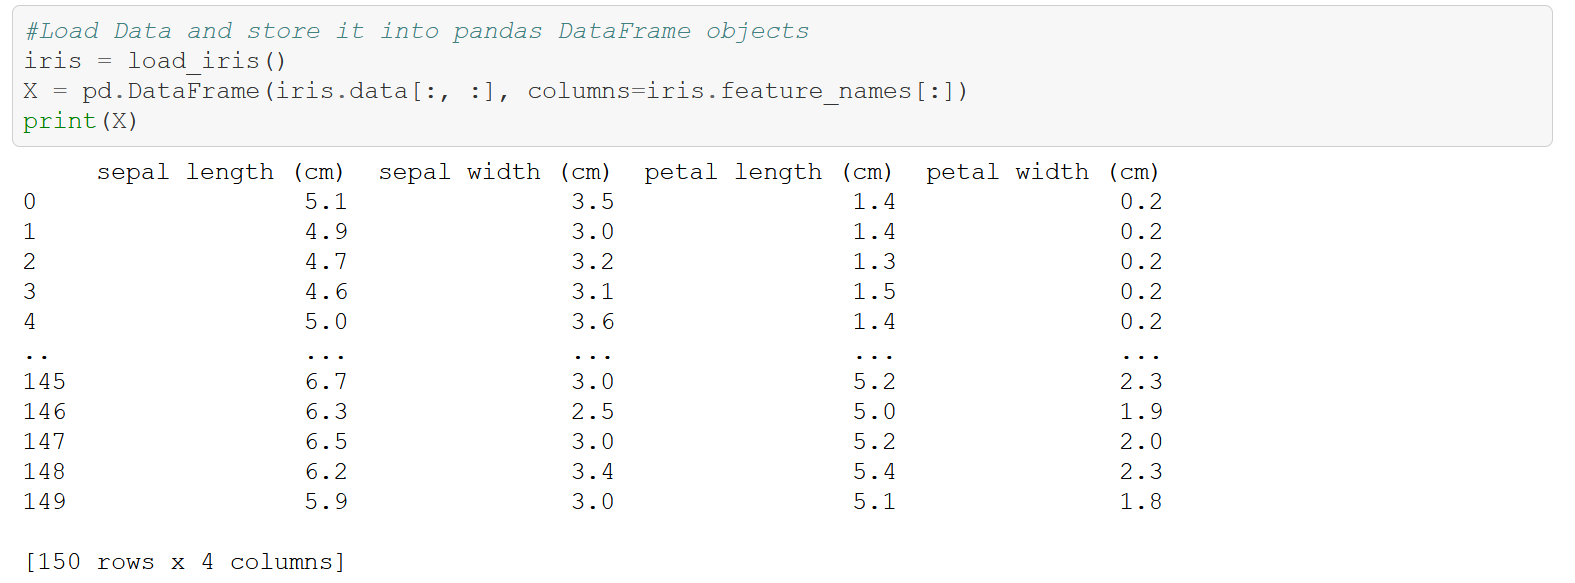
\includegraphics[width=6.8in]{1.png}
\label{fig:label}
\end{figure} 

\begin{figure}[H]
%  \centering
\caption{DATA AFTER SCALING }
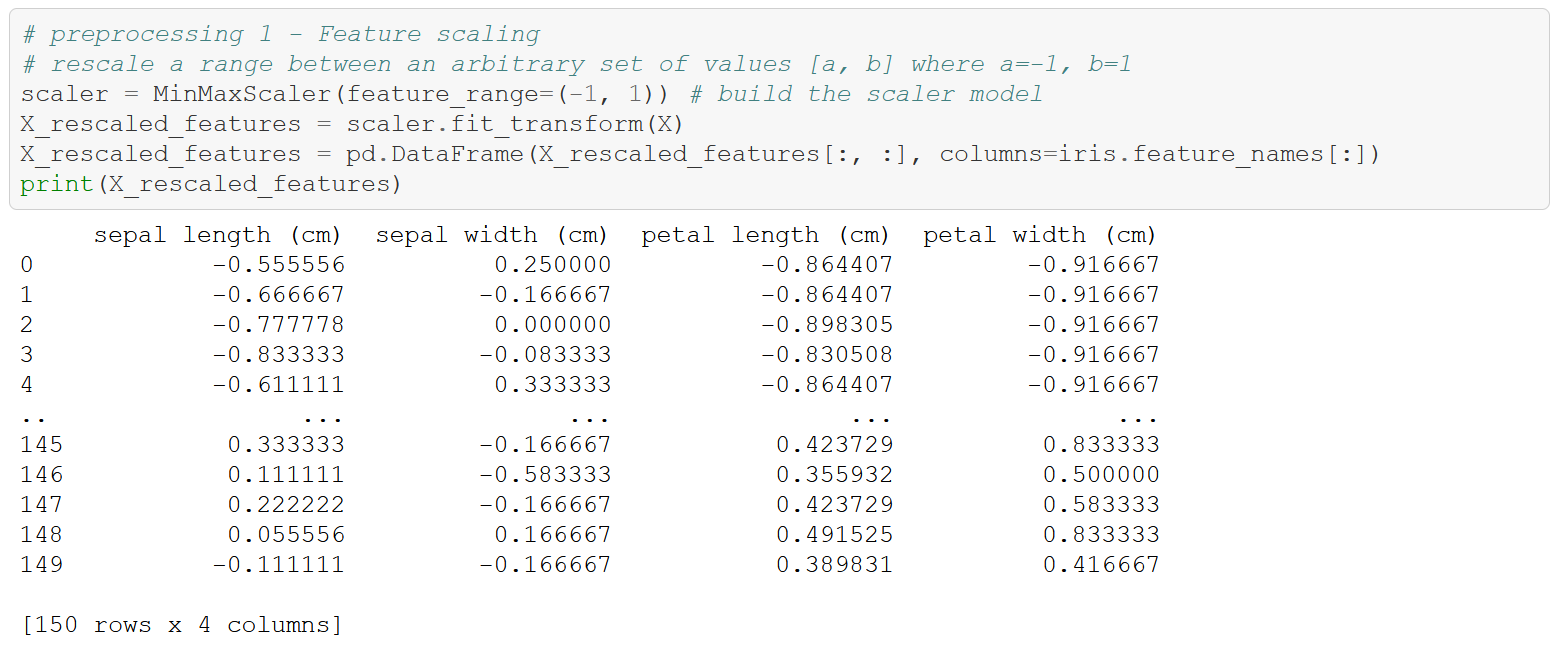
\includegraphics[width=6.8in]{2.png}
\label{fig:label}
\end{figure} 


We next use train\textunderscore test\textunderscore split model from sklearn to Split data set into random train and test subsets.\\ 
Using the train parameter we build the decision tree using DecisionTreeClassifier package from sklearn, choosing 4 as the tree's max depth. 
\subsubsection{Code}
\begin{lstlisting}
def scaling(X):
    scaler = MinMaxScaler(feature_range=(-1, 1))
    X_rescaled_features = scaler.fit_transform(X)
    return X_rescaled_features
\end{lstlisting}
\subsection{POLYNOM}


We construct a low-degree polynomial approximation in order to approximate the step function, aiming to replace it with a soft step function.\\
This is done by using mean square integral solution which is the soft step function : 
\begin{equation}
\begin{split}
\phi = \underset{p \in p_n}{min}\int\limits_{-2}^2 (I_0(x) - p(x))^2 \ dx
\end{split}
\end{equation}
 Then, by adding an importance to weight of the approximation interval we maintain the sensitivity to error in the approximation is uniform over the domain.
This leads to the optimization problem given in the article :
\begin{equation}
\begin{split}
\phi = \underset{p \in p_n}{min}\int\limits_{-2}^2 (I_0(x) - p(x))^2 w(x) \ dx
\end{split}
\end{equation}


\subsubsection{Code}
We present our code for the polynomial approximation:\\
\begin{lstlisting}
def polynom(degree, window):
    X = np.linspace(-2, 2, num=201)
    y1 = np.zeros(100)
    y2 = np.ones(101)
    Y = np.concatenate((y1, y2), axis=None)
    # weights functions
    w1 = np.concatenate((window * (np.ones(75)), np.zeros(51)), axis=None)
    w2 = window * np.ones(75)
    weight = np.concatenate((w1, w2), axis=None)
    pf = np.polyfit(X, Y, degree, w=weight)
    phi = np.poly1d(pf)
    return phi
\end{lstlisting}
\par Using sklearn numpy model we used linspace function to create an evenly spaced samples which are calculated over an interval[start,stop], the returned value is stored in parameter X.\\
Followed by parameter Y, the step function which maps the values \([1,100]\) to 0 and values \([101,201]\) to 1.
\par X represents a numpy array with values in range \([-2,2]\) with 201 samples.\\
If we choose window to be equal to 0.25 then, the array X will be divided to 3 ranges: \([-2:-0.25]\), \([-0.25:0.25]\) and \([0.25:2]\). The size of ranges \([-2:-0.25] + [0.25:2]\) is 7/2. The values in ranges \([1:75]\) and \([127:201]\) have a weight of 2/7 according to the equation:
\begin{equation}
\begin{split}
\int\limits_{-2}^2  w(x) \ dx\ = 1 
\end{split}
\end{equation}
while the values in range \([76:126]\) have weights of 0.
Using polyfit model, X is fitted to Y with degree = 34 and the calculated weights above.
\par We perform polynomial fitting on data set using polyfit model which returns a vector of coefficients p that minimizes the squared error. Then we create a polynomial model using poly1d function, which it's return value indicates whether the polynomial's coefficients powers are in a decreasing order.
The result is stored in parameter phi.


\subsection{Build Tree With 1-Hot Encoding Labels}
We start building our tree by calling the builtTree function in file my\textunderscore tree.py.\\
Each tree's inner node has a field for threshold, feature and node\textunderscore id.\\
Parameters in builtTree function :\\
lenHot = length of label's value.\\
index\textunderscore of\textunderscore max = index of argmax value.\\
Using these two parameters, leaf array is built, so it's size is equal to the size of lenHot array. It's initialized with zeros, and ones in index\textunderscore of\textunderscore max.\\
Thus, we get an array of values as a form of 1 hot encoding.\\ 
\underline{Example:} \\


\begin{figure}[H]
\centering
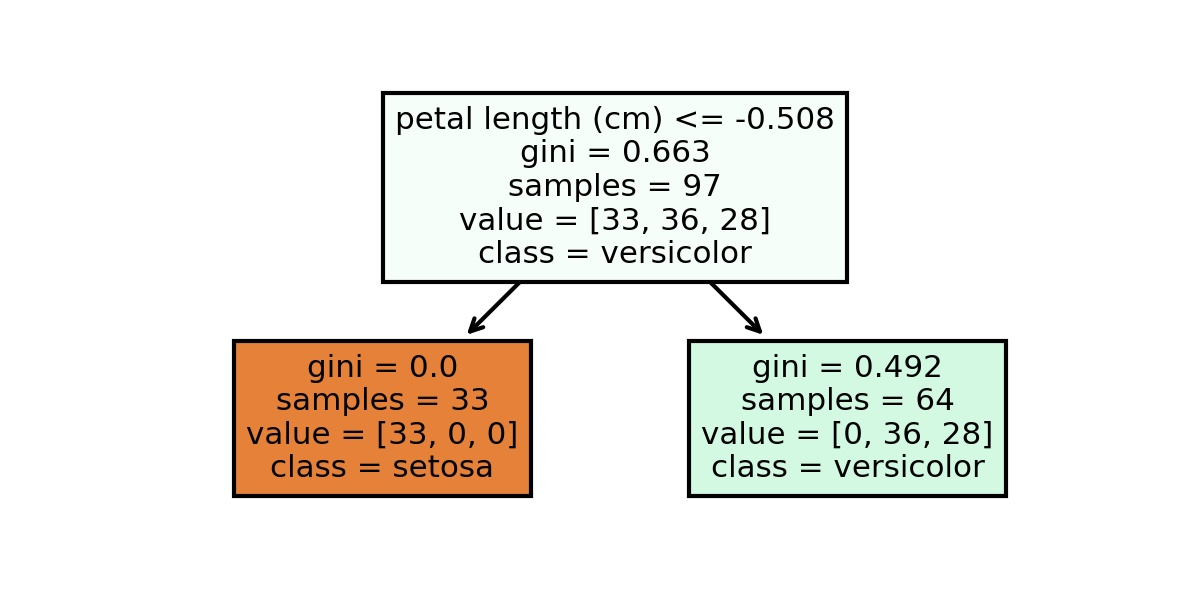
\includegraphics[width=3.5in]{one hot.jpg}
\caption{}
\label{fig:label}{Subtree labels before 1-hot encoding}
\end{figure}

\centerline{ \underline{Labels of the subtree after 1-hot encoding. }}

\centerline{leaf =  [1. 0. 0.]}

\centerline{leaf =  [0. 1. 0.]}


\underline{builtTree function}
This function receives as input, the tree and node\textunderscore id which is initialized to 0. Tree's nodes are numbered by post-order traversal.\\
Recursively, leaves values are updated to 1 hot encoding format.\\
\par
\underline{printTree function:}This function receives as input, the tree and tree's depth which is initialized to 0.\\
For every inner node, threshold and feature are printed. However, for every leaf, only 1 hot value is printed.\\
printTree function recognizes whether the node is an inner node or leaf using \(isinstance(leaf, np.ndarray)\) which returns if there's an array in the current node, if True then it's a leaf.




\section{Algorithm 1}
\subsubsection{Code}
\begin{lstlisting}
def Tree_Predict(T, x, phi):
    if T is None:
        return
    feature, threshold, leaf, left, right = T.getNode()
    if isinstance(leaf, np.ndarray):
        return leaf
    else:
        return (phi(x[feature] - threshold)) * Tree_Predict(right, x, phi) + 
        + (phi(threshold - x[feature])) * Tree_Predict(left, x, phi)
\end{lstlisting}


Akavia's algorithm traverses all paths in the tree and computes a weighted combination of
all the leaves values, where each leaf value is the 1-hot encoding of the
label associated with the leaf. The output is a length L vector assigning a
likelihood score to each label, which is in turn interpreted as outputting
the label with the highest score.\\
Here we used polyval 



\section{Accuracy}

The accuracy is calculated as the percentage of correct classification on test samples. \\
\begin{lstlisting}
algorithm1_score = (counter / len(res_vec))*100 
\end{lstlisting}

Counter is equal to the sum of correct classifications and res\_vec is equal to the sum of all classifications.\\ 
To know if current classification is correct or not we compare it to Y target value of the relevant sample if they are eqaul then the prediction of algorithm 1 is correct . \\

test samples are decided to sent to algorithm 1 as 35\% of the samples in the data-set and they are chosen randomly from the data-set.\\
test samples are assigned to variable X\_test. \\
So algorithm 1 predict over all test samples, after that we calculate accuracy according to the percentage of correct predictions on test samples that algorithm 1 predict.\\

\begin{lstlisting}
for x in X_test:
    res = algorithm1_predict(myTree, x, phi)
    res_vec.append(res)
\end{lstlisting}

\newpage
\textcolor{red}{We trained trees up to depth 6 and compare algorithm 1 prediction's accuracy vs. scikit learn prediction's accuracy for three data sets: iris, wine and cancer.}\\

\begin{multicols}{2}

\begin{table}[H]
\caption{ iris}
\label{tab:my-table}
\begin{tabular}{|l|l|l|}


\hline
\textbf{Tree depth} & Algorithm 1 acc & scikit learn acc \\ \hline
\textbf{0} & 22.64151 & 22.64151 \\ \hline
\textbf{1} & 62.26415 & 62.26415 \\ \hline
\textbf{2} & 94.33962 & 94.33962 \\ \hline
\textbf{3} & 86.7925 & 96.22642 \\ \hline
\textbf{4} & 100 & 96.22642 \\ \hline
\textbf{5} & 94.3396 & 96.22642 \\ \hline
\textbf{6} & 98.1132 & 94.33962 \\ \hline
\end{tabular}
\end{table}

\begin{figure}[H]
\centering
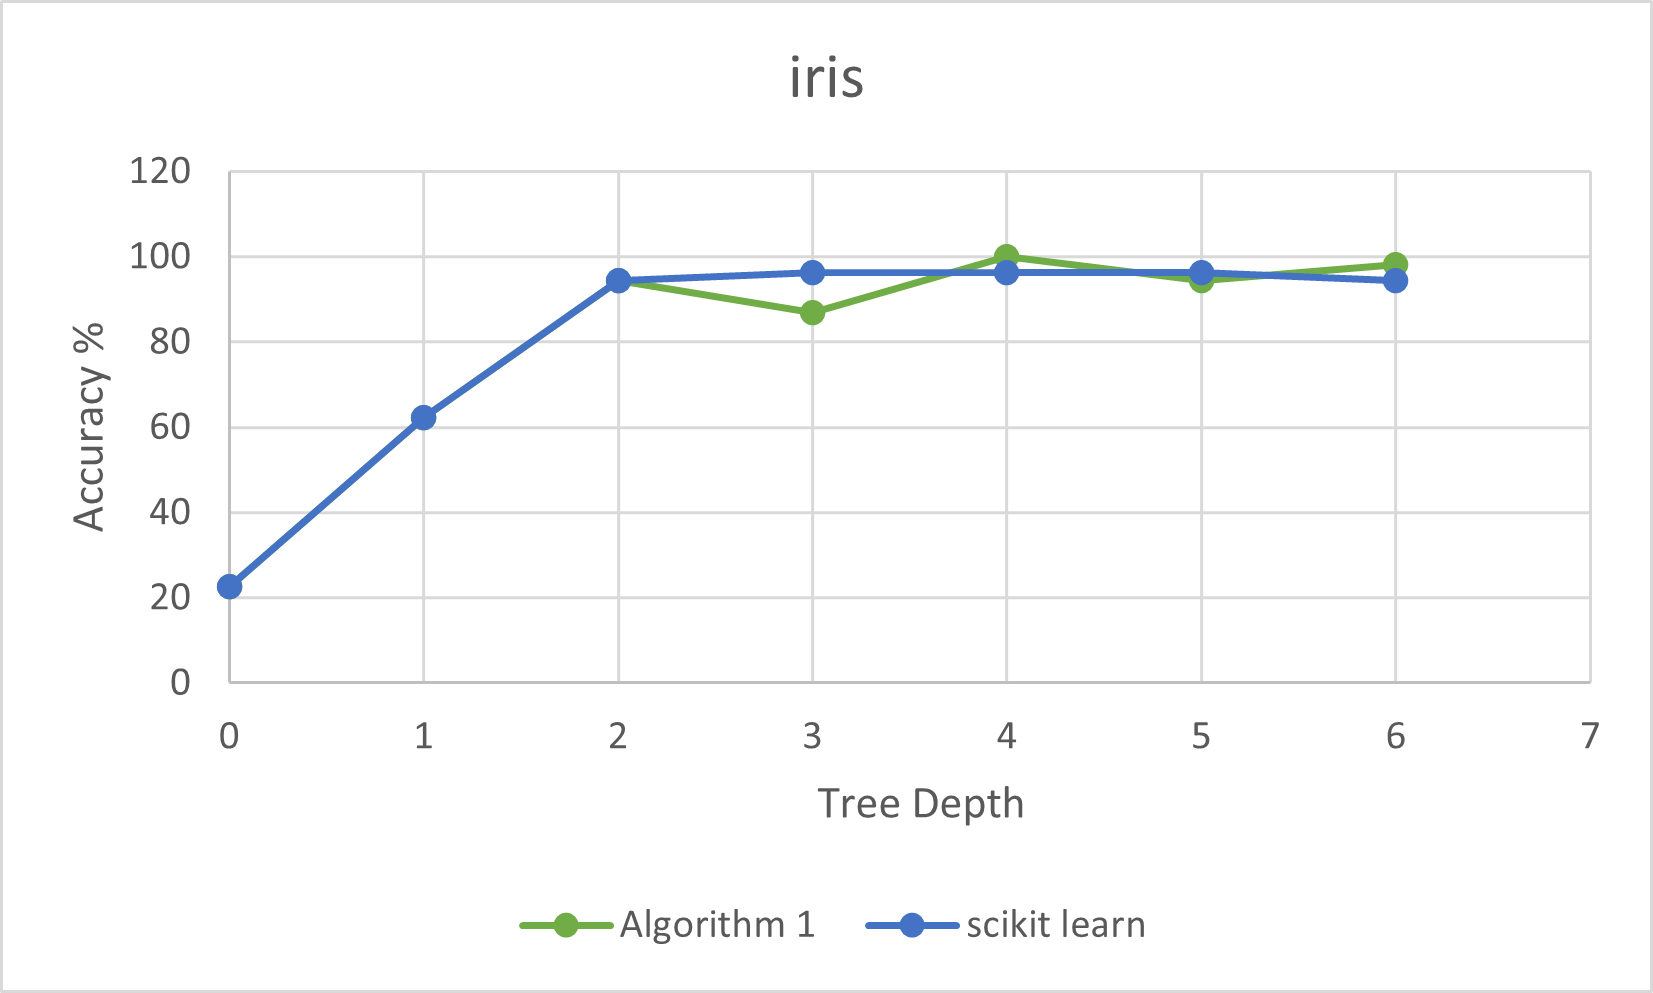
\includegraphics[width=3.5in]{iris_acc.png}
\caption{}
\label{fig:label}{Accuracy of ours vs. Scikit-learn on iris dataset and tree depth 0-6}
\end{figure}
\end{multicols}


\begin{multicols}{2}



\begin{table}[H]
\caption{ wine}
\label{tab:my-table}
\begin{tabular}{|l|l|l|}
\hline
\textbf{Tree depth} & Algorithm 1 acc & scikit learn acc \\ \hline
\textbf{0} & 38.09524 & 38.09524 \\ \hline
\textbf{1} & 50.79365 & 50.79365 \\ \hline
\textbf{2} & 90.4762 & 87.30159 \\ \hline
\textbf{3} & 92.0635 & 90.47619 \\ \hline
\textbf{4} & 90.4762 & 88.88889 \\ \hline
\textbf{5} & 93.6508 & 92.06349 \\ \hline
\textbf{6} & 96.8254 & 92.06349 \\ \hline
\end{tabular}
\end{table}

\begin{figure}[H]
\centering
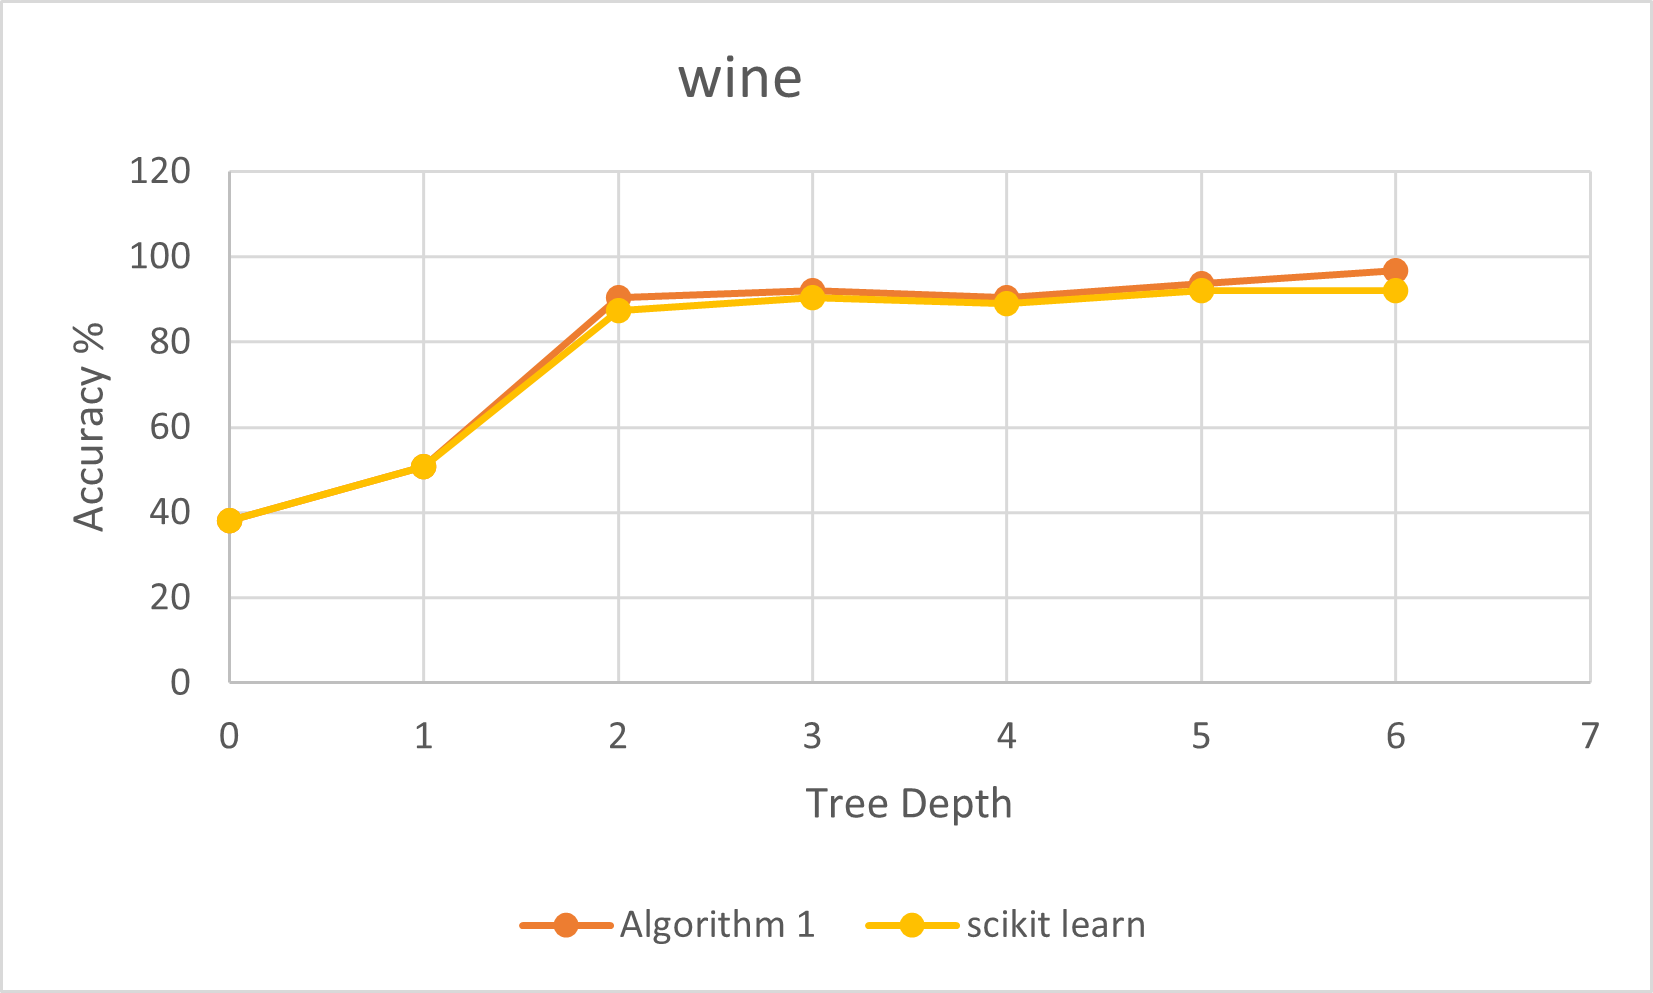
\includegraphics[width=3.5in]{wine_acc.png}
\caption{}
\label{fig:label}{Accuracy of ours vs. Scikit-learn on Wine dataset and tree depth 0-6}
\end{figure}
\end{multicols}

\begin{multicols}{2}
\begin{table}[H]
\caption{ cnacer}
\label{tab:my-table}
\begin{tabular}{|l|l|l|}
\hline
\textbf{Tree depth} & Algorithm 1 acc & scikit learn acc \\ \hline
\textbf{0} & 61.5 & 61.5 \\ \hline
\textbf{1} & 87.5 & 87.5 \\ \hline
\textbf{2} & 94.5 & 91 \\ \hline
\textbf{3} & 96 & 96 \\ \hline
\textbf{4} & 94.5 & 91.5 \\ \hline
\textbf{5} & 92 & 92 \\ \hline
\textbf{6} & 96.5 & 92 \\ \hline
\end{tabular}
\end{table}

\begin{figure}[H]
\centering
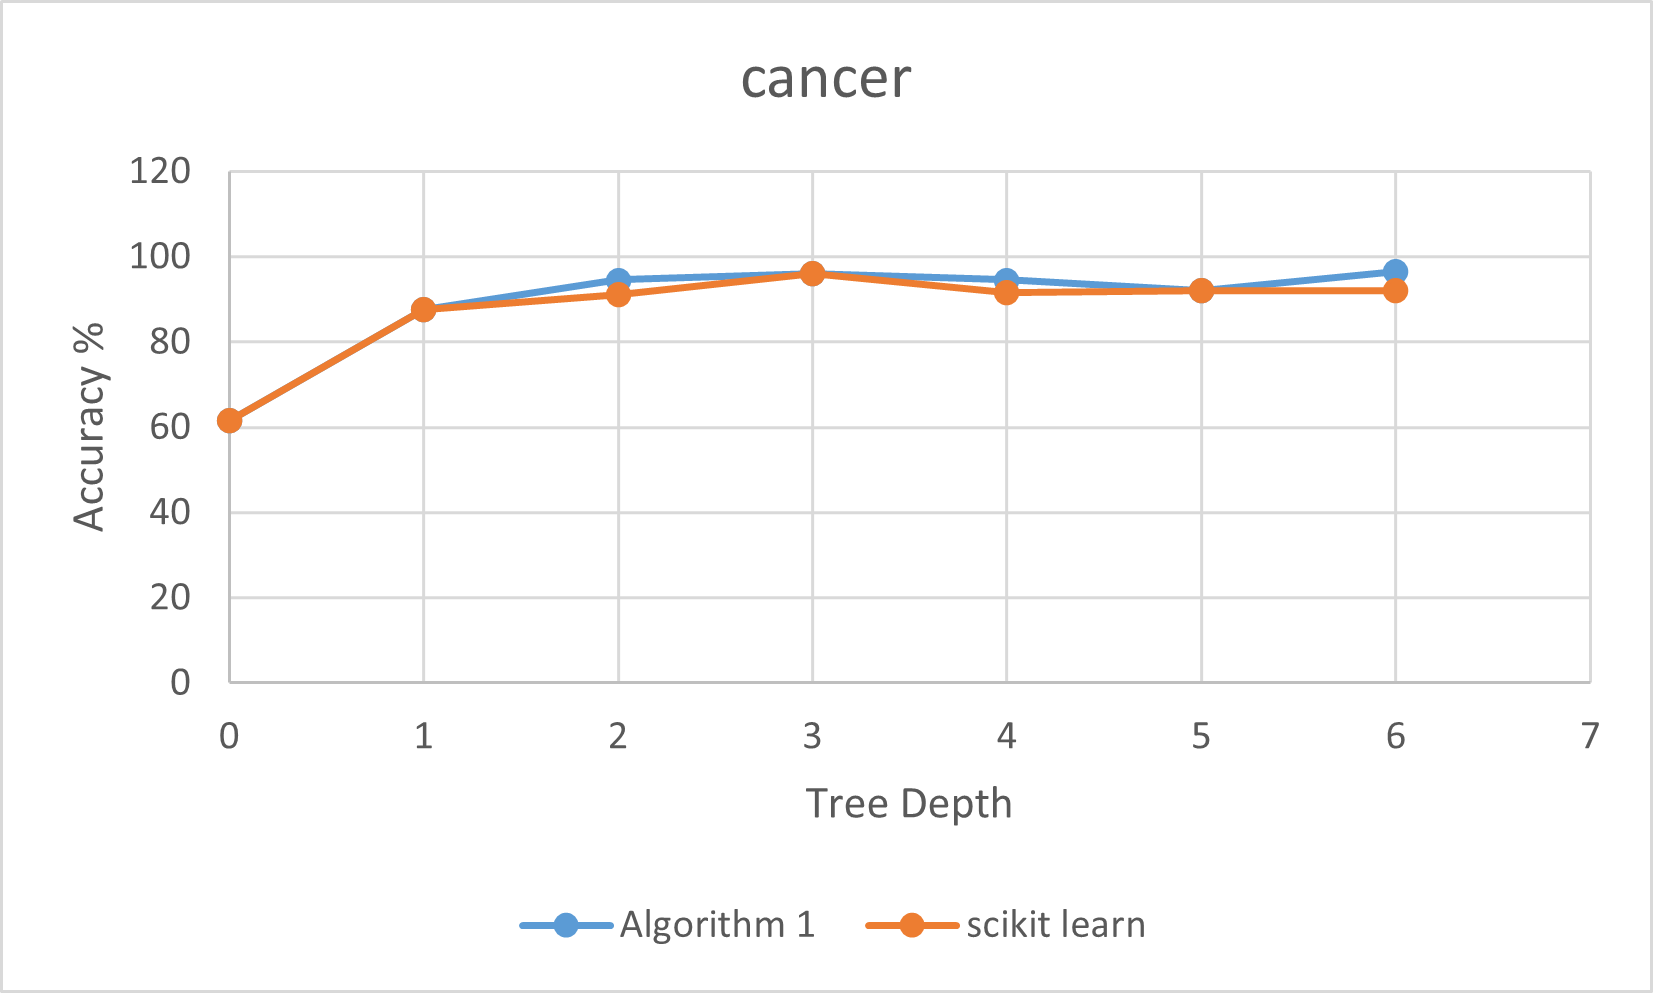
\includegraphics[width=3.5in]{cancer_acc.png}
\caption{}
\label{fig:label}{Accuracy of ours vs. Scikit-learn on Cancer dataset and tree depth 0-6}
\end{figure}
\end{multicols}





\newpage
\section{Results}
\underline{\large{Example of results we got :}}
\begin{multicols}{2}
data\_type = iris\\
max depth = 4\\
scikit\_learn\_score = 92.45283 \% \\\\
WINDOW = 0 \\\\
window = 0\\
polynom order = 0\\
run time = 0.0180 seconds\\
algorithm1\_score = 32.0755 \%\\
-----------------------------------------\\
window = 0\\
polynom order = 1\\
run time =0.0150 seconds\\
algorithm1\_score = 90.5660 \%\\
-----------------------------------------\\
window = 0\\
polynom order = 2\\
run time =0.0180 seconds\\
algorithm1\_score = 90.5660 \%\\
-----------------------------------------\\
window = 0 \\
polynom order = 3\\
run time = 0.0190 seconds\\
algorithm1\_score = 92.4528 \%\\
-----------------------------------------\\
.\\
.\\
.\\
window = 0\\
polynom order = 33\\
run time = 0.0349 seconds\\
algorithm1\_score = 92.4528 \% \\\\
-----------------------------------------\\
WINDOW = 0.25\\\\
window = 0.25\\
polynom order = 0\\
run time = 0.0439 seconds\\
algorithm1\_score = 32.0755 \%\\
\\
.\\
.\\
.\\
window = 0.25\\
polynom order = 33\\
run time = 0.0499 seconds\\
algorithm1\_score = 92.4528 \%\\
\\
-----------------------------------------\\
WINDOW = 0.5 \\\\
window = 0.5\\
polynom order = 0\\
run time = 0.0429 seconds\\
algorithm1\_score = 32.0755 \%\\
\\
.\\
.\\
.\\
window = 0.5\\
polynom order = 33\\
run time = 0.0499 seconds\\
algorithm1\_score = 92.4528 \%\\
\\
-----------------------------------------\\
WINDOW = 0.75 \\\\
window = 0.75\\
polynom order = 0\\
run time = 0.0259 seconds\\
algorithm1\_score = 32.0755 \%\\
\\
.\\
.\\
.\\
window = 0.75\\
polynom order = 33\\
run time = 0.0289 seconds\\
algorithm1\_score = 92.4528 \%\\
\end{multicols}

\textbf{For each window \(\textbf{[0, 0.25, 0.5, 0.75]}\) We calculate the algorithm's 1 accuracy for every polynom's degree in range [0,33]. \\ 
Then we arranged all the results in tables ( table 4 to 15).} \\

\newpage
\subsection{Results For Cancer Data-Set}

%  Cancer tree
\underline{\large{Cancer Tree:}}\\ \\
\hspace*{0pt}feature =  22  threshold =  -0.41192\\
\hspace*{15pt}feature =  27  threshold =  0.28384\\
\hspace*{25pt}feature =  27  threshold =  -0.23814\\
\hspace*{40pt} feature =  28  threshold =  -0.99980\\
\hspace*{55pt}leaf =  [1. 0.] \\
\hspace*{55pt}leaf =  [0. 1.] \\
\hspace*{40pt}feature =  1 threshold =  -0.23266\\
\hspace*{55pt}leaf =  [0. 1.] \\
\hspace*{55pt}leaf =  [1. 0.] \\
\hspace*{25pt}leaf =  [1. 0.]\\
\hspace*{15pt}feature =  6 threshold =  -0.65742\\
\hspace*{25pt}feature =  1 threshold =  -0.38282\\
\hspace*{40pt}leaf =  [0. 1.]\\
\hspace*{40pt} feature =  15 threshold =  -0.72109\\
\hspace*{55pt}leaf =  [1. 0.] \\
\hspace*{55pt}leaf =  [0. 1.] \\
\hspace*{25pt}feature =  7 threshold =  -0.57465\\
\hspace*{40pt} feature =  9 threshold =  -0.49326\\
\hspace*{55pt}leaf =  [1. 0.] \\
\hspace*{55pt}leaf =  [0. 1.] \\
\hspace*{40pt}feature =  1 threshold =  -0.70172\\
\hspace*{55pt}leaf =  [1. 0.] \\
\hspace*{55pt}leaf =  [1. 0.] \\


% cancer tree figure

\begin{figure}[H]
\centering
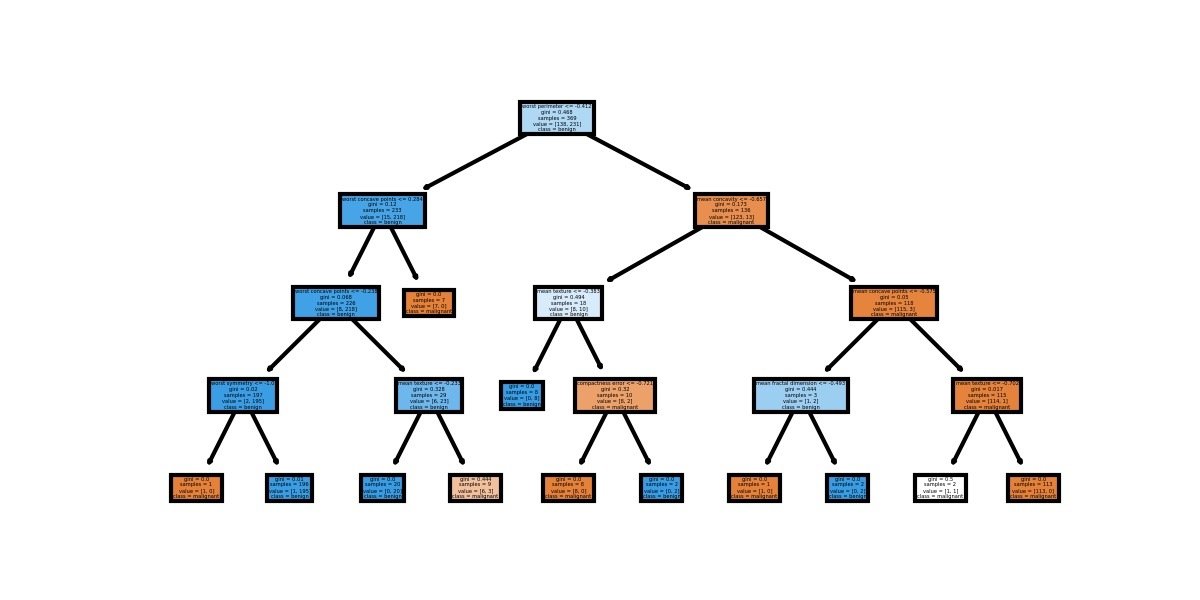
\includegraphics[width=8.5in]{cancer.jpg}
\caption{Cancer Tree Figure (Before 1 Hot Encoding) With Max Depth = 4 }
\label{fig_error}
\end{figure}


\newpage
\begin{multicols}{2}

% Table 1
\begin{table}[H]
\caption{}
\label{tab:my-table}
\begin{tabular}{|c|c|c|c|}
\hline
\multicolumn{4}{|c|}{\textbf{Dataset: Cancer}} \\ \hline
\multicolumn{4}{|c|}{\textbf{scikit learn score = 94.50000  \%}} \\ \hline
\multicolumn{4}{|c|}{\textbf{max depth = 4}} \\ \hline
Window & Polynom Degree & Runtime (sec) & Score (\%) \\ \hline
 & 0 & 0.0788 & 37 \\ \cline{2-4} 
 & 1 & 0.0798 &  \\ \cline{2-3}
 & 2 & 0.0927 & \multirow{-2}{*}{75.5} \\ \cline{2-4} 
 & 3 & 0.1087 &  \\ \cline{2-3}
 & 4 & 0.1077 & \multirow{-2}{*}{92} \\ \cline{2-4} 
 & 5 & 0.1197 &  \\ \cline{2-3}
 & 6 & 0.1137 & \multirow{-2}{*}{92.5} \\ \cline{2-4} 
 & 7 & 0.1117 &  \\ \cline{2-3}
 & 8 & 0.1137 &  \\ \cline{2-3}
 & 9 & 0.1177 &  \\ \cline{2-3}
 & 10 & 0.1027 & \multirow{-4}{*}{95.5} \\ \cline{2-4} 
 & 11 & 0.1137 &  \\ \cline{2-3}
 & 12 & 0.1117 & \multirow{-2}{*}{96} \\ \cline{2-4} 
 & 13 & 0.1167 &  \\ \cline{2-3}
 & 14 & 0.1117 & \multirow{-2}{*}{96.5} \\ \cline{2-4} 
 & \cellcolor[HTML]{FFFFC7}15 & \cellcolor[HTML]{FFFFC7}0.1227 & \cellcolor[HTML]{FFFFC7} \\ \cline{2-3}
 & 16 & 0.1206 & \multirow{-2}{*}{\cellcolor[HTML]{FFFFC7}97} \\ \cline{2-4} 
 & 17 & 0.1316 &  \\ \cline{2-3}
 & 18 & 0.1326 &  \\ \cline{2-3}
 & 19 & 0.1247 &  \\ \cline{2-3}
 & 20 & 0.1426 & \multirow{-4}{*}{96.5} \\ \cline{2-4} 
 & 21 & 0.1416 &  \\ \cline{2-3}
 & 22 & 0.1326 & \multirow{-2}{*}{96} \\ \cline{2-4} 
 & 23 & 0.1277 &  \\ \cline{2-3}
 & 24 & 0.1526 & \multirow{-2}{*}{96.5} \\ \cline{2-4} 
 & 25 & 0.1307 &  \\ \cline{2-3}
 & 26 & 0.1735 &  \\ \cline{2-3}
 & 27 & 0.1706 &  \\ \cline{2-3}
 & 28 & 0.167 &  \\ \cline{2-3}
 & 29 & 0.128 &  \\ \cline{2-3}
 & 30 & 0.148 &  \\ \cline{2-3}
 & 31 & 0.152 &  \\ \cline{2-3}
 & 32 & 0.156 &  \\ \cline{2-3}
\multirow{-34}{*}{0} & 33 & 0.144 & \multirow{-9}{*}{96} \\ \hline
\end{tabular}
\end{table}


\begin{table}[H]
\caption{}
\label{tab:my-table}
\begin{tabular}{|c|c|c|c|}
\hline
\multicolumn{4}{|c|}{\textbf{Dataset: Cancer}} \\ \hline
\multicolumn{4}{|c|}{\textbf{scikit learn score =94.50000  \%}} \\ \hline
\multicolumn{4}{|c|}{\textbf{max depth = 4}} \\ \hline
Window & Polynom Degree & Runtime (sec)& Score (\%) \\ \hline
 & 0 & 0.084 & 37 \\ \cline{2-4} 
 & 1 & 0.08 &  \\ \cline{2-3}
 & 2 & 0.104 & \multirow{-2}{*}{75.5} \\ \cline{2-4} 
 & 3 & 0.1 &  \\ \cline{2-3}
 & 4 & 0.092 & \multirow{-2}{*}{92} \\ \cline{2-4} 
 & 5 & 0.104 &  \\ \cline{2-3}
 & 6 & 0.104 & \multirow{-2}{*}{92.5} \\ \cline{2-4} 
 & 7 & 0.092 &  \\ \cline{2-3}
 & 8 & 0.116 &  \\ \cline{2-3}
 & 9 & 0.096 &  \\ \cline{2-3}
 & 10 & 0.1 & \multirow{-4}{*}{95.5} \\ \cline{2-4} 
 & 11 & 0.12 &  \\ \cline{2-3}
 & 12 & 0.104 & \multirow{-2}{*}{96} \\ \cline{2-4} 
 & 13 & 0.12 &  \\ \cline{2-3}
 & 14 & 0.128 & \multirow{-2}{*}{96.5} \\ \cline{2-4} 
 & \cellcolor[HTML]{FFFFC7}15 & \cellcolor[HTML]{FFFFC7}0.108 & \cellcolor[HTML]{FFFFC7} \\ \cline{2-3}
 & 16 & 0.12 & \multirow{-2}{*}{\cellcolor[HTML]{FFFFC7}97} \\ \cline{2-4} 
 & 17 & 0.12 &  \\ \cline{2-3}
 & 18 & 0.144 &  \\ \cline{2-3}
 & 19 & 0.128 &  \\ \cline{2-3}
 & 20 & 0.128 & \multirow{-4}{*}{96.5} \\ \cline{2-4} 
 & 21 & 0.124 &  \\ \cline{2-3}
 & 22 & 0.136 & \multirow{-2}{*}{96} \\ \cline{2-4} 
 & 23 & 0.144 &  \\ \cline{2-3}
 & 24 & 0.124 & \multirow{-2}{*}{96.5} \\ \cline{2-4} 
 & 25 & 0.164 &  \\ \cline{2-3}
 & 26 & 0.136 &  \\ \cline{2-3}
 & 27 & 0.14 &  \\ \cline{2-3}
 & 28 & 0.136 &  \\ \cline{2-3}
 & 29 & 0.144 &  \\ \cline{2-3}
 & 30 & 0.132 &  \\ \cline{2-3}
 & 31 & 0.152 &  \\ \cline{2-3}
 & 32 & 0.168 &  \\ \cline{2-3}
\multirow{-34}{*}{0.25} & 33 & 0.16 & \multirow{-9}{*}{96} \\ \hline
\end{tabular}
\end{table}

\begin{table}[H]
\caption{}
\label{tab:my-table}
\begin{tabular}{|c|c|c|c|}
\hline
\multicolumn{4}{|c|}{Dataset: Cancer} \\ \hline
\multicolumn{4}{|c|}{\textbf{scikit learn score = 94.50000  \%}} \\ \hline
\multicolumn{4}{|c|}{\textbf{max depth = 4}} \\ \hline
Window & Polynom Degree & Runtime (sec) & Score (\%) \\ \hline
 & 0 & 0.08 & 37 \\ \cline{2-4} 
 & 1 & 0.104 &  \\ \cline{2-3}
 & 2 & 0.08 & \multirow{-2}{*}{75.5} \\ \cline{2-4} 
 & 3 & 0.104 &  \\ \cline{2-3}
 & 4 & 0.092 & \multirow{-2}{*}{92} \\ \cline{2-4} 
 & 5 & 0.084 &  \\ \cline{2-3}
 & 6 & 0.112 & \multirow{-2}{*}{92.5} \\ \cline{2-4} 
 & 7 & 0.1 &  \\ \cline{2-3}
 & 8 & 0.096 &  \\ \cline{2-3}
 & 9 & 0.12 &  \\ \cline{2-3}
 & 10 & 0.096 & \multirow{-4}{*}{95.5} \\ \cline{2-4} 
 & 11 & 0.104 &  \\ \cline{2-3}
 & 12 & 0.124 & \multirow{-2}{*}{96} \\ \cline{2-4} 
 & 13 & 0.1 &  \\ \cline{2-3}
 & 14 & 0.1 & \multirow{-2}{*}{96.5} \\ \cline{2-4} 
 & \cellcolor[HTML]{FFFFC7}15 & \cellcolor[HTML]{FFFFC7}0.2 & \cellcolor[HTML]{FFFFC7} \\ \cline{2-3}
 & 16 & 0.128 & \multirow{-2}{*}{\cellcolor[HTML]{FFFFC7}97} \\ \cline{2-4} 
 & 17 & 0.132 &  \\ \cline{2-3}
 & 18 & 0.116 &  \\ \cline{2-3}
 & 19 & 0.136 &  \\ \cline{2-3}
 & 20 & 0.124 & \multirow{-4}{*}{96.5} \\ \cline{2-4} 
 & 21 & 0.12 &  \\ \cline{2-3}
 & 22 & 0.136 & \multirow{-2}{*}{96} \\ \cline{2-4} 
 & 23 & 0.14 &  \\ \cline{2-3}
 & 24 & 0.14 & \multirow{-2}{*}{96.5} \\ \cline{2-4} 
 & 25 & 0.136 &  \\ \cline{2-3}
 & 26 & 0.132 &  \\ \cline{2-3}
 & 27 & 0.136 &  \\ \cline{2-3}
 & 28 & 0.14 &  \\ \cline{2-3}
 & 29 & 0.156 &  \\ \cline{2-3}
 & 30 & 0.148 &  \\ \cline{2-3}
 & 31 & 0.16 &  \\ \cline{2-3}
 & 32 & 0.148 &  \\ \cline{2-3}
\multirow{-34}{*}{0.5} & 33 & 0.152 & \multirow{-9}{*}{96} \\ \hline
\end{tabular}
\end{table}


\begin{table}[H]
\caption{}
\label{tab:my-table}
\begin{tabular}{|c|c|c|c|}
\hline
\multicolumn{4}{|c|}{\textbf{Dataset: Cancer}} \\ \hline
\multicolumn{4}{|c|}{\textbf{scikit learn score = 94.50000  \%}} \\ \hline
\multicolumn{4}{|c|}{\textbf{max depth = 4}} \\ \hline
Window & Polynom Degree & Runtime (sec) & Score (\%) \\ \hline
 & 0 & 0.084 & 37 \\ \cline{2-4} 
 & 1 & 0.1 &  \\ \cline{2-3}
 & 2 & 0.08 & \multirow{-2}{*}{75.5} \\ \cline{2-4} 
 & 3 & 0.108 &  \\ \cline{2-3}
 & 4 & 0.088 & \multirow{-2}{*}{92} \\ \cline{2-4} 
 & 5 & 0.084 &  \\ \cline{2-3}
 & 6 & 0.104 & \multirow{-2}{*}{92.5} \\ \cline{2-4} 
 & 7 & 0.104 &  \\ \cline{2-3}
 & 8 & 0.092 &  \\ \cline{2-3}
 & 9 & 0.116 &  \\ \cline{2-3}
 & 10 & 0.104 & \multirow{-4}{*}{95.5} \\ \cline{2-4} 
 & 11 & 0.112 &  \\ \cline{2-3}
 & 12 & 0.104 & \multirow{-2}{*}{96} \\ \cline{2-4} 
 & 13 & 0.144 &  \\ \cline{2-3}
 & 14 & 0.12 & \multirow{-2}{*}{96.5} \\ \cline{2-4} 
 & \cellcolor[HTML]{FFFFC7}15 & \cellcolor[HTML]{FFFFC7}0.12 & \cellcolor[HTML]{FFFFC7} \\ \cline{2-3}
 & 16 & 0.112 & \multirow{-2}{*}{\cellcolor[HTML]{FFFFC7}97} \\ \cline{2-4} 
 & 17 & 0.124 &  \\ \cline{2-3}
 & 18 & 0.128 &  \\ \cline{2-3}
 & 19 & 0.128 &  \\ \cline{2-3}
 & 20 & 0.124 & \multirow{-4}{*}{96.5} \\ \cline{2-4} 
 & 21 & 0.14 &  \\ \cline{2-3}
 & 22 & 0.156 & \multirow{-2}{*}{96} \\ \cline{2-4} 
 & 23 & 0.1721 &  \\ \cline{2-3}
 & 24 & 0.1728 & \multirow{-2}{*}{96.5} \\ \cline{2-4} 
 & 25 & 0.1754 &  \\ \cline{2-3}
 & 26 & 0.1767 &  \\ \cline{2-3}
 & 27 & 0.1746 &  \\ \cline{2-3}
 & 28 & 0.2059 &  \\ \cline{2-3}
 & 29 & 0.1549 &  \\ \cline{2-3}
 & 30 & 0.156 &  \\ \cline{2-3}
 & 31 & 0.136 &  \\ \cline{2-3}
 & 32 & 0.156 &  \\ \cline{2-3}
\multirow{-34}{*}{0.75} & 33 & 0.148 & \multirow{-9}{*}{96} \\ \hline
\end{tabular}
\end{table}


\end{multicols}
\newpage
\subsection{Results For Iris Data-Set}
% \begin{multicols}{2}
% Iris tree
\underline{\large{Iris Tree:}}\\ \\
\hspace*{0pt}feature =  2 threshold =  -0.45762\\
\hspace*{15pt}leaf =  [1. 0. 0.]\\
\hspace*{15pt}feature =  2 threshold =  0.30508\\
\hspace*{25pt}feature =  3 threshold =  0.29166\\
\hspace*{40pt}leaf =  [0. 1. 0.]\\
\hspace*{40pt}feature =  1 threshold =  -0.08333\\
\hspace*{50pt}leaf =  [0. 0. 1.]\\
\hspace*{50pt}leaf =  [0. 1. 0.]\\
\hspace*{25pt}feature =  3 threshold =  0.33333\\
\hspace*{40pt}feature =  0 threshold =  -0.02777\\
\hspace*{50pt}leaf =  [0. 1. 0.]\\
\hspace*{50pt}leaf =  [0. 0. 1.]\\
\hspace*{40pt}leaf =  [0. 0. 1.]\\
% \begin{multicols}{2}
% Iris tree figure
\begin{figure}[H]

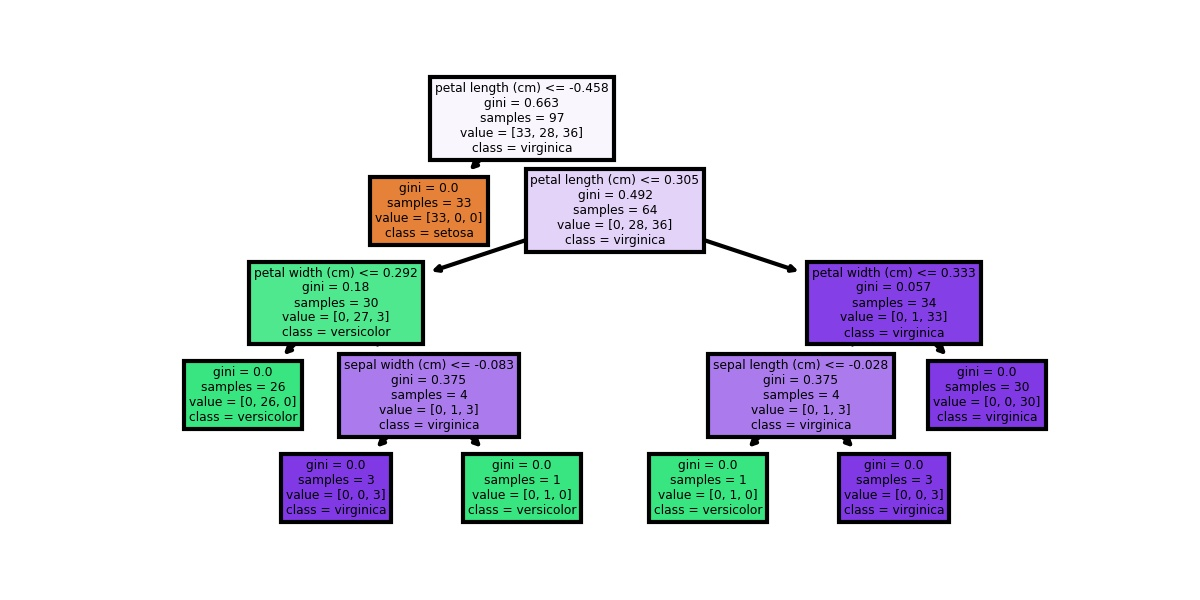
\includegraphics[width=8.5in]{iris tree.jpg}
\caption{Iris Tree Figure (Before 1 Hot Encoding) With Max Depth = 4 }
% \label{fig_error}
\end{figure} 
% \end{multicols}

\newpage
\begin{multicols}{2}
% window = 0 / iris
\begin{table}[H]
\caption{}
\label{tab:my-table}
\begin{tabular}{|c|c|c|c|}
\hline
\multicolumn{4}{|c|}{\textbf{Dataset: Iris}} \\ \hline
\multicolumn{4}{|c|}{\textbf{scikit learn score = 92.45283\%}} \\ \hline
\multicolumn{4}{|c|}{\textbf{max depth = 4}} \\ \hline
Window & Polynom Degree & Runtime (sec) & Score (\%) \\ \hline
 & 0 & 0.018 & 32.0755 \\ \cline{2-4} 
 & 1 & 0.015 &  \\ \cline{2-3}
 & 2 & 0.018 & \multirow{-2}{*}{90.566} \\ \cline{2-4} 
 & 3 & 0.019 &  \\ \cline{2-3}
 & 4 & 0.016 &  \\ \cline{2-3}
 & 5 & 0.0279 &  \\ \cline{2-3}
 & 6 & 0.018 &  \\ \cline{2-3}
 & 7 & 0.017 &  \\ \cline{2-3}
 & 8 & 0.017 & \multirow{-6}{*}{92.4528} \\ \cline{2-4} 
 & \cellcolor[HTML]{FFFFC7}9 & \cellcolor[HTML]{FFFFC7}0.016 & \cellcolor[HTML]{FFFFC7} \\ \cline{2-3}
 & 10 & 0.015 & \cellcolor[HTML]{FFFFC7} \\ \cline{2-3}
 & 11 & 0.0159 & \cellcolor[HTML]{FFFFC7} \\ \cline{2-3}
 & 12 & 0.015 & \multirow{-4}{*}{\cellcolor[HTML]{FFFFC7}94.3396} \\ \cline{2-4} 
 & 13 & 0.0189 &  \\ \cline{2-3}
 & 14 & 0.019 &  \\ \cline{2-3}
 & 15 & 0.0239 &  \\ \cline{2-3}
 & 16 & 0.0199 &  \\ \cline{2-3}
 & 17 & 0.0249 &  \\ \cline{2-3}
 & 18 & 0.018 &  \\ \cline{2-3}
 & 19 & 0.0179 &  \\ \cline{2-3}
 & 20 & 0.0209 &  \\ \cline{2-3}
 & 21 & 0.0189 &  \\ \cline{2-3}
 & 22 & 0.0209 &  \\ \cline{2-3}
 & 23 & 0.0249 &  \\ \cline{2-3}
 & 24 & 0.0309 &  \\ \cline{2-3}
 & 25 & 0.0259 &  \\ \cline{2-3}
 & 26 & 0.024 &  \\ \cline{2-3}
 & 27 & 0.0219 &  \\ \cline{2-3}
 & 28 & 0.0209 &  \\ \cline{2-3}
 & 29 & 0.0219 &  \\ \cline{2-3}
 & 30 & 0.02 &  \\ \cline{2-3}
 & 31 & 0.0219 &  \\ \cline{2-3}
 & 32 & 0.0299 &  \\ \cline{2-3}
\multirow{-34}{*}{0} & 33 & 0.0349 & \multirow{-21}{*}{92.4528} \\ \hline
\end{tabular}
\end{table}

% window = 0.25 / iris

\begin{table}[H]
\caption{}
\label{tab:my-table}
\begin{tabular}{|c|c|c|c|}
\hline
\multicolumn{4}{|c|}{\textbf{Dataset: Iris}} \\ \hline
\multicolumn{4}{|c|}{\textbf{scikit learn score = 92.45283\%}} \\ \hline
\multicolumn{4}{|c|}{\textbf{max depth = 4}} \\ \hline
\textbf{Window} & \textbf{Polynom Degree} & \textbf{Runtime (sec)} & \textbf{Score (\%)} \\ \hline
 & 0 & 0.0439 & 32.0755 \\ \cline{2-4} 
 & 1 & 0.0259 &  \\ \cline{2-3}
 & 2 & 0.017 & \multirow{-2}{*}{90.566} \\ \cline{2-4} 
 & 3 & 0.0149 &  \\ \cline{2-3}
 & 4 & 0.016 &  \\ \cline{2-3}
 & 5 & 0.0289 &  \\ \cline{2-3}
 & 6 & 0.0339 &  \\ \cline{2-3}
 & 7 & 0.0229 &  \\ \cline{2-3}
 & 8 & 0.0289 & \multirow{-6}{*}{92.4528} \\ \cline{2-4} 
 & \cellcolor[HTML]{FFFFC7}9 & \cellcolor[HTML]{FFFFC7}0.0299 & \cellcolor[HTML]{FFFFC7} \\ \cline{2-3}
 & 10 & 0.0369 & \cellcolor[HTML]{FFFFC7} \\ \cline{2-3}
 & 11 & 0.0219 & \cellcolor[HTML]{FFFFC7} \\ \cline{2-3}
 & 12 & 0.0279 & \multirow{-4}{*}{\cellcolor[HTML]{FFFFC7}94.3396} \\ \cline{2-4} 
 & 13 & 0.0439 &  \\ \cline{2-3}
 & 14 & 0.0329 &  \\ \cline{2-3}
 & 15 & 0.0489 &  \\ \cline{2-3}
 & 16 & 0.0379 &  \\ \cline{2-3}
 & 17 & 0.0349 &  \\ \cline{2-3}
 & 18 & 0.0219 &  \\ \cline{2-3}
 & 19 & 0.0189 &  \\ \cline{2-3}
 & 20 & 0.0209 &  \\ \cline{2-3}
 & 21 & 0.0219 &  \\ \cline{2-3}
 & 22 & 0.0209 &  \\ \cline{2-3}
 & 23 & 0.0489 &  \\ \cline{2-3}
 & 24 & 0.1007 &  \\ \cline{2-3}
 & 25 & 0.0718 &  \\ \cline{2-3}
 & 26 & 0.0349 &  \\ \cline{2-3}
 & 27 & 0.0349 &  \\ \cline{2-3}
 & 28 & 0.0479 &  \\ \cline{2-3}
 & 29 & 0.0329 &  \\ \cline{2-3}
 & 30 & 0.0449 &  \\ \cline{2-3}
 & 31 & 0.0349 &  \\ \cline{2-3}
 & 32 & 0.0559 &  \\ \cline{2-3}
\multirow{-34}{*}{0.25} & 33 & 0.0499 & \multirow{-21}{*}{92.4528} \\ \hline
\end{tabular}
\end{table}

% window = 0.5 / iris

\begin{table}[H]
\caption{}
\label{tab:my-table}
\begin{tabular}{|c|c|c|c|}
\hline
\multicolumn{4}{|c|}{\textbf{Dataset: Iris}} \\ \hline
\multicolumn{4}{|c|}{\textbf{scikit learn score = 92.45283\%}} \\ \hline
\multicolumn{4}{|c|}{\textbf{max depth = 4}} \\ \hline
Window & Polynom Degree & Runtime (sec) & Score (\%) \\ \hline
 & 0 & 0.0429 & 32.0755 \\ \cline{2-4} 
 & 1 & 0.022 &  \\ \cline{2-3}
 & 2 & 0.0229 & \multirow{-2}{*}{90.566} \\ \cline{2-4} 
 & 3 & 0.0209 &  \\ \cline{2-3}
 & 4 & 0.0199 &  \\ \cline{2-3}
 & 5 & 0.0219 &  \\ \cline{2-3}
 & 6 & 0.0239 &  \\ \cline{2-3}
 & 7 & 0.0219 &  \\ \cline{2-3}
 & 8 & 0.0329 & \multirow{-6}{*}{92.4528} \\ \cline{2-4} 
 & \cellcolor[HTML]{FFFFC7}9 & \cellcolor[HTML]{FFFFC7}0.0249 & \cellcolor[HTML]{FFFFC7} \\ \cline{2-3}
 & 10 & 0.0249 & \cellcolor[HTML]{FFFFC7} \\ \cline{2-3}
 & 11 & 0.0379 & \cellcolor[HTML]{FFFFC7} \\ \cline{2-3}
 & 12 & 0.0349 & \multirow{-4}{*}{\cellcolor[HTML]{FFFFC7}94.3396} \\ \cline{2-4} 
 & 13 & 0.0299 &  \\ \cline{2-3}
 & 14 & 0.0239 &  \\ \cline{2-3}
 & 15 & 0.0239 &  \\ \cline{2-3}
 & 16 & 0.0319 &  \\ \cline{2-3}
 & 17 & 0.0279 &  \\ \cline{2-3}
 & 18 & 0.0219 &  \\ \cline{2-3}
 & 19 & 0.0219 &  \\ \cline{2-3}
 & 20 & 0.0199 &  \\ \cline{2-3}
 & 21 & 0.0189 &  \\ \cline{2-3}
 & 22 & 0.0748 &  \\ \cline{2-3}
 & 23 & 0.1237 &  \\ \cline{2-3}
 & 24 & 0.0219 &  \\ \cline{2-3}
 & 25 & 0.0259 &  \\ \cline{2-3}
 & 26 & 0.0229 &  \\ \cline{2-3}
 & 27 & 0.0279 &  \\ \cline{2-3}
 & 28 & 0.0249 &  \\ \cline{2-3}
 & 29 & 0.0239 &  \\ \cline{2-3}
 & 30 & 0.0279 &  \\ \cline{2-3}
 & 31 & 0.0349 &  \\ \cline{2-3}
 & 32 & 0.026 &  \\ \cline{2-3}
\multirow{-34}{*}{0.5} & 33 & 0.0209 & \multirow{-21}{*}{92.4528} \\ \hline
\end{tabular}
\end{table}

% window = 0.75 / iris

\begin{table}[H]
\caption{}
\label{tab:my-table}
\begin{tabular}{|c|c|c|c|}
\hline
\multicolumn{4}{|c|}{\textbf{Dataset: Iris}} \\ \hline
\multicolumn{4}{|c|}{\textbf{scikit learn score = 92.45283\%}} \\ \hline
\multicolumn{4}{|c|}{\textbf{max depth = 4}} \\ \hline
Window & Polynom Degree & Runtime (sec) & Score (\%) \\ \hline
 & 0 & 0.0259 & 32.0755 \\ \cline{2-4} 
 & 1 & 0.0319 &  \\ \cline{2-3}
 & 2 & 0.0269 & \multirow{-2}{*}{90.566} \\ \cline{2-4} 
 & 3 & 0.0279 &  \\ \cline{2-3}
 & 4 & 0.0309 &  \\ \cline{2-3}
 & 5 & 0.0299 &  \\ \cline{2-3}
 & 6 & 0.0269 &  \\ \cline{2-3}
 & 7 & 0.0239 &  \\ \cline{2-3}
 & 8 & 0.0199 & \multirow{-6}{*}{92.4528} \\ \cline{2-4} 
 & \cellcolor[HTML]{FFFFC7}9 & \cellcolor[HTML]{FFFFC7}0.0319 & \cellcolor[HTML]{FFFFC7} \\ \cline{2-3}
 & 10 & 0.0239 & \cellcolor[HTML]{FFFFC7} \\ \cline{2-3}
 & 11 & 0.0199 & \cellcolor[HTML]{FFFFC7} \\ \cline{2-3}
 & 12 & 0.0279 & \multirow{-4}{*}{\cellcolor[HTML]{FFFFC7}94.3396} \\ \cline{2-4} 
 & 13 & 0.0219 &  \\ \cline{2-3}
 & 14 & 0.02 &  \\ \cline{2-3}
 & 15 & 0.0249 &  \\ \cline{2-3}
 & 16 & 0.0229 &  \\ \cline{2-3}
 & 17 & 0.0239 &  \\ \cline{2-3}
 & 18 & 0.0229 &  \\ \cline{2-3}
 & 19 & 0.0219 &  \\ \cline{2-3}
 & 20 & 0.0239 &  \\ \cline{2-3}
 & 21 & 0.0239 &  \\ \cline{2-3}
 & 22 & 0.0219 &  \\ \cline{2-3}
 & 23 & 0.0349 &  \\ \cline{2-3}
 & 24 & 0.0369 &  \\ \cline{2-3}
 & 25 & 0.0419 &  \\ \cline{2-3}
 & 26 & 0.0299 &  \\ \cline{2-3}
 & 27 & 0.0279 &  \\ \cline{2-3}
 & 28 & 0.0289 &  \\ \cline{2-3}
 & 29 & 0.0369 &  \\ \cline{2-3}
 & 30 & 0.0399 &  \\ \cline{2-3}
 & 31 & 0.0309 &  \\ \cline{2-3}
 & 32 & 0.0269 &  \\ \cline{2-3}
\multirow{-34}{*}{0.75} & 33 & 0.0289 & \multirow{-21}{*}{92.4528} \\ \hline
\end{tabular}
\end{table}
\end{multicols}
\newpage
\subsection{Results For Wine Data-Set}

\underline{\large{Wine Tree:}}\\ \\
\hspace*{0pt}feature =  6 threshold =  -0.16877\\
\hspace*{15pt}feature =  9 threshold =  -0.56569\\
\hspace*{25pt}leaf =  [0. 1. 0.] \\
\hspace*{25pt}feature =  6 threshold =  -0.55274\\
\hspace*{40pt}leaf =  [0. 0. 1.] \\
\hspace*{40pt}feature =  10 threshold =  -0.61788\\
\hspace*{55pt}leaf =  [0. 0. 1.] \\
\hspace*{55pt}leaf =  [0. 1. 0.] \\
\hspace*{15pt}feature =  12 threshold =  -0.36305\\
\hspace*{25pt}feature =  1 threshold =  0.23320\\
\hspace*{40pt}leaf =  [0. 1. 0.] \\
\hspace*{40pt}leaf =  [1. 0. 0.] \\
\hspace*{25pt}feature =  4 threshold =  0.42391\\
\hspace*{40pt}leaf =  [1. 0. 0.] \\
\hspace*{40pt}leaf =  [0. 1. 0.] \\


% wine tree figure
\begin{figure}[H]

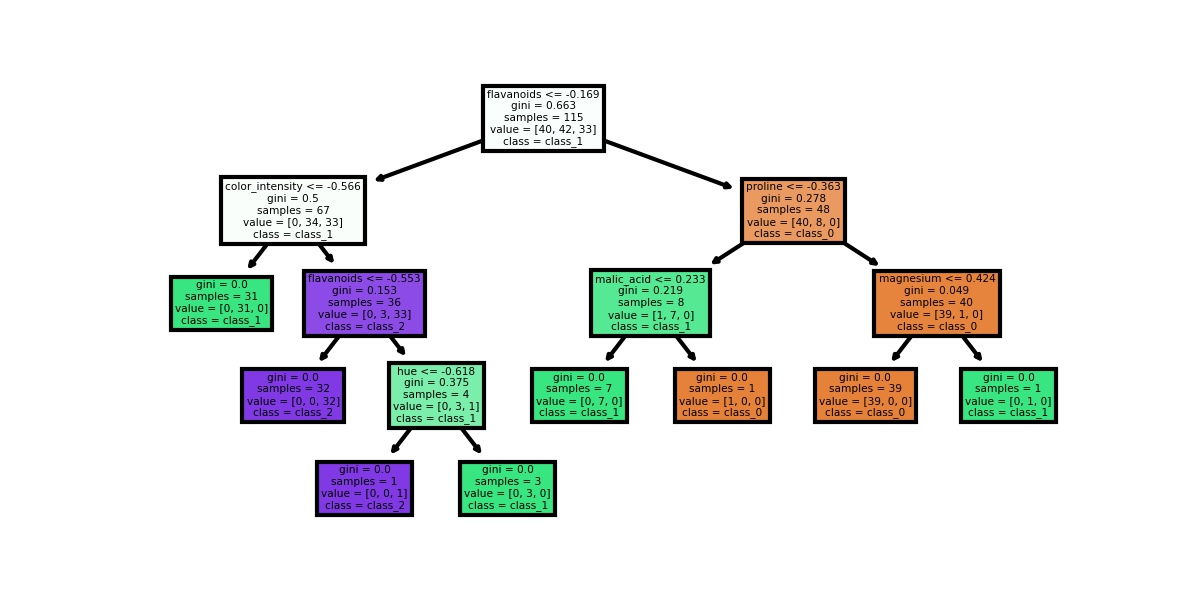
\includegraphics[width=7.5in]{wine tree.jpg}
\caption{Wine Tree Figure (Before 1 Hot Encoding) With Max Depth = 4 }
% \label{fig_error}
\end{figure} 


\newpage
\begin{multicols}{2}
\begin{table}[H]
\caption{}
\label{tab:my-table}
\begin{tabular}{|c|c|c|c|}
\hline
\multicolumn{4}{|c|}{\textbf{Dataset: Wine}} \\ \hline
\multicolumn{4}{|c|}{scikit learn score = 93.65079 \%} \\ \hline
\multicolumn{4}{|c|}{max depth = 4} \\ \hline
Window & Polynom Degree & Runtime (sec) & Score (\%) \\ \hline
 & 0 & 0.0152 & 46.0317 \\ \cline{2-4} 
 & 1 & 0.0112 &  \\ \cline{2-3}
 & 2 & 0.0126 & \multirow{-2}{*}{55.5556} \\ \cline{2-4} 
 & 3 & 0.0116 &  \\ \cline{2-3}
 & 4 & 0.0126 & \multirow{-2}{*}{76.1905} \\ \cline{2-4} 
 & 5 & 0.012 &  \\ \cline{2-3}
 & 6 & 0.0122 & \multirow{-2}{*}{84.127} \\ \cline{2-4} 
 & 7 & 0.0124 &  \\ \cline{2-3}
 & 8 & 0.0127 &  \\ \cline{2-3}
 & 9 & 0.0247 &  \\ \cline{2-3}
 & 10 & 0.0225 & \multirow{-4}{*}{92.0635} \\ \cline{2-4} 
 & \cellcolor[HTML]{FFFFC7}11 & \cellcolor[HTML]{FFFFC7}0.0203 & \cellcolor[HTML]{FFFFC7} \\ \cline{2-3}
 & 12 & 0.0176 & \cellcolor[HTML]{FFFFC7} \\ \cline{2-3}
 & 13 & 0.0178 & \cellcolor[HTML]{FFFFC7} \\ \cline{2-3}
 & 14 & 0.0175 & \cellcolor[HTML]{FFFFC7} \\ \cline{2-3}
 & 15 & 0.0157 & \cellcolor[HTML]{FFFFC7} \\ \cline{2-3}
 & 16 & 0.0145 & \cellcolor[HTML]{FFFFC7} \\ \cline{2-3}
 & 17 & 0.0147 & \cellcolor[HTML]{FFFFC7} \\ \cline{2-3}
 & 18 & 0.0148 & \cellcolor[HTML]{FFFFC7} \\ \cline{2-3}
 & 19 & 0.0152 & \cellcolor[HTML]{FFFFC7} \\ \cline{2-3}
 & 20 & 0.0155 & \cellcolor[HTML]{FFFFC7} \\ \cline{2-3}
 & 21 & 0.022 & \cellcolor[HTML]{FFFFC7} \\ \cline{2-3}
 & 22 & 0.0219 & \cellcolor[HTML]{FFFFC7} \\ \cline{2-3}
 & 23 & 0.0193 & \cellcolor[HTML]{FFFFC7} \\ \cline{2-3}
 & 24 & 0.0225 & \cellcolor[HTML]{FFFFC7} \\ \cline{2-3}
 & 25 & 0.0235 & \cellcolor[HTML]{FFFFC7} \\ \cline{2-3}
 & 26 & 0.0178 & \cellcolor[HTML]{FFFFC7} \\ \cline{2-3}
 & 27 & 0.0167 & \cellcolor[HTML]{FFFFC7} \\ \cline{2-3}
 & 28 & 0.0166 & \cellcolor[HTML]{FFFFC7} \\ \cline{2-3}
 & 29 & 0.0172 & \cellcolor[HTML]{FFFFC7} \\ \cline{2-3}
 & 30 & 0.0173 & \cellcolor[HTML]{FFFFC7} \\ \cline{2-3}
 & 31 & 0.0173 & \cellcolor[HTML]{FFFFC7} \\ \cline{2-3}
 & 32 & 0.0233 & \cellcolor[HTML]{FFFFC7} \\ \cline{2-3}
 & 33 & 0.0226 & \cellcolor[HTML]{FFFFC7} \\ \cline{2-3}
\multirow{-35}{*}{0} & 34 & 0.0234 & \multirow{-24}{*}{\cellcolor[HTML]{FFFFC7}95.2381} \\ \hline
\end{tabular}
\end{table}


\begin{table}[H]
\caption{}
\label{tab:my-table}
\begin{tabular}{|c|c|c|c|}
\hline
\multicolumn{4}{|c|}{\textbf{Dataset: Wine}} \\ \hline
\multicolumn{4}{|c|}{\textbf{scikit learn score = 93.65079 \%}} \\ \hline
\multicolumn{4}{|c|}{\textbf{max depth = 4}} \\ \hline
Window & Polynom Degree & Runtime (sec) & Score (\%) \\ \hline
 & 0 & 0.0159 & 46.0317 \\ \cline{2-4} 
 & 1 & 0.0135 &  \\ \cline{2-3}
 & 2 & 0.0146 & \multirow{-2}{*}{55.5556} \\ \cline{2-4} 
 & 3 & 0.0131 &  \\ \cline{2-3}
 & 4 & 0.012 & \multirow{-2}{*}{76.1905} \\ \cline{2-4} 
 & 5 & 0.0124 &  \\ \cline{2-3}
 & 6 & 0.0123 & \multirow{-2}{*}{84.127} \\ \cline{2-4} 
 & 7 & 0.0126 &  \\ \cline{2-3}
 & 8 & 0.0131 &  \\ \cline{2-3}
 & 9 & 0.0131 &  \\ \cline{2-3}
 & 10 & 0.0154 & \multirow{-4}{*}{92.0635} \\ \cline{2-4} 
 & \cellcolor[HTML]{FFFFC7}11 & \cellcolor[HTML]{FFFFC7}0.0196 & \cellcolor[HTML]{FFFFC7} \\ \cline{2-3}
 & 12 & 0.0175 & \cellcolor[HTML]{FFFFC7} \\ \cline{2-3}
 & 13 & 0.0187 & \cellcolor[HTML]{FFFFC7} \\ \cline{2-3}
 & 14 & 0.0202 & \cellcolor[HTML]{FFFFC7} \\ \cline{2-3}
 & 15 & 0.0187 & \cellcolor[HTML]{FFFFC7} \\ \cline{2-3}
 & 16 & 0.017 & \cellcolor[HTML]{FFFFC7} \\ \cline{2-3}
 & 17 & 0.0148 & \cellcolor[HTML]{FFFFC7} \\ \cline{2-3}
 & 18 & 0.0149 & \cellcolor[HTML]{FFFFC7} \\ \cline{2-3}
 & 19 & 0.0153 & \cellcolor[HTML]{FFFFC7} \\ \cline{2-3}
 & 20 & 0.0153 & \cellcolor[HTML]{FFFFC7} \\ \cline{2-3}
 & 21 & 0.0152 & \cellcolor[HTML]{FFFFC7} \\ \cline{2-3}
 & 22 & 0.0221 & \cellcolor[HTML]{FFFFC7} \\ \cline{2-3}
 & 23 & 0.0205 & \cellcolor[HTML]{FFFFC7} \\ \cline{2-3}
 & 24 & 0.0226 & \cellcolor[HTML]{FFFFC7} \\ \cline{2-3}
 & 25 & 0.0205 & \cellcolor[HTML]{FFFFC7} \\ \cline{2-3}
 & 26 & 0.02 & \cellcolor[HTML]{FFFFC7} \\ \cline{2-3}
 & 27 & 0.0169 & \cellcolor[HTML]{FFFFC7} \\ \cline{2-3}
 & 28 & 0.0167 & \cellcolor[HTML]{FFFFC7} \\ \cline{2-3}
 & 29 & 0.0173 & \cellcolor[HTML]{FFFFC7} \\ \cline{2-3}
 & 30 & 0.0176 & \cellcolor[HTML]{FFFFC7} \\ \cline{2-3}
 & 31 & 0.0174 & \cellcolor[HTML]{FFFFC7} \\ \cline{2-3}
 & 32 & 0.0175 & \cellcolor[HTML]{FFFFC7} \\ \cline{2-3}
 & 33 & 0.0254 & \cellcolor[HTML]{FFFFC7} \\ \cline{2-3}
\multirow{-35}{*}{0.25} & 34 & 0.027 & \multirow{-24}{*}{\cellcolor[HTML]{FFFFC7}95.2381} \\ \hline
\end{tabular}
\end{table}

% Please add the following required packages to your document preamble:
% \usepackage{multirow}
% \usepackage[table,xcdraw]{xcolor}
% If you use beamer only pass "xcolor=table" option, i.e. \documentclass[xcolor=table]{beamer}
\begin{table}[H]
\caption{}
\label{tab:my-table}
\begin{tabular}{|c|c|c|c|}
\hline
\multicolumn{4}{|c|}{\textbf{Dataset: Wine}} \\ \hline
\multicolumn{4}{|c|}{\textbf{scikit learn score = 93.65079 \%}} \\ \hline
\multicolumn{4}{|c|}{\textbf{max depth = 4}} \\ \hline
Window & Polynom Degree & Runtime (sec) & Score (\%) \\ \hline
 & 0 & 0.0147 & 46.0317 \\ \cline{2-4} 
 & 1 & 0.0259 &  \\ \cline{2-3}
 & 2 & 0.025 & \multirow{-2}{*}{55.5556} \\ \cline{2-4} 
 & 3 & 0.0165 &  \\ \cline{2-3}
 & 4 & 0.0123 & \multirow{-2}{*}{76.1905} \\ \cline{2-4} 
 & 5 & 0.0128 &  \\ \cline{2-3}
 & 6 & 0.0132 & \multirow{-2}{*}{84.127} \\ \cline{2-4} 
 & 7 & 0.0134 &  \\ \cline{2-3}
 & 8 & 0.0136 &  \\ \cline{2-3}
 & 9 & 0.0136 &  \\ \cline{2-3}
 & 10 & 0.0212 & \multirow{-4}{*}{92.0635} \\ \cline{2-4} 
 & \cellcolor[HTML]{FFFFC7}11 & \cellcolor[HTML]{FFFFC7}0.0159 & \cellcolor[HTML]{FFFFC7} \\ \cline{2-3}
 & 12 & 0.0165 & \cellcolor[HTML]{FFFFC7} \\ \cline{2-3}
 & 13 & 0.0182 & \cellcolor[HTML]{FFFFC7} \\ \cline{2-3}
 & 14 & 0.0173 & \cellcolor[HTML]{FFFFC7} \\ \cline{2-3}
 & 15 & 0.0238 & \cellcolor[HTML]{FFFFC7} \\ \cline{2-3}
 & 16 & 0.0153 & \cellcolor[HTML]{FFFFC7} \\ \cline{2-3}
 & 17 & 0.0152 & \cellcolor[HTML]{FFFFC7} \\ \cline{2-3}
 & 18 & 0.0156 & \cellcolor[HTML]{FFFFC7} \\ \cline{2-3}
 & 19 & 0.016 & \cellcolor[HTML]{FFFFC7} \\ \cline{2-3}
 & 20 & 0.0162 & \cellcolor[HTML]{FFFFC7} \\ \cline{2-3}
 & 21 & 0.0206 & \cellcolor[HTML]{FFFFC7} \\ \cline{2-3}
 & 22 & 0.0191 & \cellcolor[HTML]{FFFFC7} \\ \cline{2-3}
 & 23 & 0.0214 & \cellcolor[HTML]{FFFFC7} \\ \cline{2-3}
 & 24 & 0.0243 & \cellcolor[HTML]{FFFFC7} \\ \cline{2-3}
 & 25 & 0.0215 & \cellcolor[HTML]{FFFFC7} \\ \cline{2-3}
 & 26 & 0.0185 & \cellcolor[HTML]{FFFFC7} \\ \cline{2-3}
 & 27 & 0.0178 & \cellcolor[HTML]{FFFFC7} \\ \cline{2-3}
 & 28 & 0.0174 & \cellcolor[HTML]{FFFFC7} \\ \cline{2-3}
 & 29 & 0.0176 & \cellcolor[HTML]{FFFFC7} \\ \cline{2-3}
 & 30 & 0.0179 & \cellcolor[HTML]{FFFFC7} \\ \cline{2-3}
 & 31 & 0.0182 & \cellcolor[HTML]{FFFFC7} \\ \cline{2-3}
 & 32 & 0.0249 & \cellcolor[HTML]{FFFFC7} \\ \cline{2-3}
 & 33 & 0.0227 & \cellcolor[HTML]{FFFFC7} \\ \cline{2-3}
\multirow{-35}{*}{0.5} & 34 & 0.0202 & \multirow{-24}{*}{\cellcolor[HTML]{FFFFC7}95.2381} \\ \hline
\end{tabular}
\end{table}


\begin{table}[H]
\caption{}
\label{tab:my-table}
\begin{tabular}{|c|c|c|c|}
\hline
\multicolumn{4}{|c|}{\textbf{Dataset: Wine}} \\ \hline
\multicolumn{4}{|c|}{\textbf{scikit learn score = 93.65079 \%}} \\ \hline
\multicolumn{4}{|c|}{\textbf{max depth = 4}} \\ \hline
Window & Polynom Degree & Runtime (sec) & Score (\%) \\ \hline
 & 0 & 0.0122 & 46.0317 \\ \cline{2-4} 
 & 1 & 0.0144 &  \\ \cline{2-3}
 & 2 & 0.0149 & \multirow{-2}{*}{55.5556} \\ \cline{2-4} 
 & 3 & 0.0125 &  \\ \cline{2-3}
 & 4 & 0.0119 & \multirow{-2}{*}{76.1905} \\ \cline{2-4} 
 & 5 & 0.0121 &  \\ \cline{2-3}
 & 6 & 0.0121 & \multirow{-2}{*}{84.127} \\ \cline{2-4} 
 & 7 & 0.0124 &  \\ \cline{2-3}
 & 8 & 0.0126 &  \\ \cline{2-3}
 & 9 & 0.0129 &  \\ \cline{2-3}
 & 10 & 0.013 & \multirow{-4}{*}{92.0635} \\ \cline{2-4} 
 & \cellcolor[HTML]{FFFFC7}11 & \cellcolor[HTML]{FFFFC7}0.0175 & \cellcolor[HTML]{FFFFC7} \\ \cline{2-3}
 & 12 & 0.0185 & \cellcolor[HTML]{FFFFC7} \\ \cline{2-3}
 & 13 & 0.0197 & \cellcolor[HTML]{FFFFC7} \\ \cline{2-3}
 & 14 & 0.0173 & \cellcolor[HTML]{FFFFC7} \\ \cline{2-3}
 & 15 & 0.0184 & \cellcolor[HTML]{FFFFC7} \\ \cline{2-3}
 & 16 & 0.0211 & \cellcolor[HTML]{FFFFC7} \\ \cline{2-3}
 & 17 & 0.0165 & \cellcolor[HTML]{FFFFC7} \\ \cline{2-3}
 & 18 & 0.0163 & \cellcolor[HTML]{FFFFC7} \\ \cline{2-3}
 & 19 & 0.0161 & \cellcolor[HTML]{FFFFC7} \\ \cline{2-3}
 & 20 & 0.0159 & \cellcolor[HTML]{FFFFC7} \\ \cline{2-3}
 & 21 & 0.016 & \cellcolor[HTML]{FFFFC7} \\ \cline{2-3}
 & 22 & 0.0161 & \cellcolor[HTML]{FFFFC7} \\ \cline{2-3}
 & 23 & 0.0198 & \cellcolor[HTML]{FFFFC7} \\ \cline{2-3}
 & 24 & 0.0217 & \cellcolor[HTML]{FFFFC7} \\ \cline{2-3}
 & 25 & 0.0219 & \cellcolor[HTML]{FFFFC7} \\ \cline{2-3}
 & 26 & 0.023 & \cellcolor[HTML]{FFFFC7} \\ \cline{2-3}
 & 27 & 0.0239 & \cellcolor[HTML]{FFFFC7} \\ \cline{2-3}
 & 28 & 0.0172 & \cellcolor[HTML]{FFFFC7} \\ \cline{2-3}
 & 29 & 0.0178 & \cellcolor[HTML]{FFFFC7} \\ \cline{2-3}
 & 30 & 0.0173 & \cellcolor[HTML]{FFFFC7} \\ \cline{2-3}
 & 31 & 0.0176 & \cellcolor[HTML]{FFFFC7} \\ \cline{2-3}
 & 32 & 0.0178 & \cellcolor[HTML]{FFFFC7} \\ \cline{2-3}
 & 33 & 0.0258 & \cellcolor[HTML]{FFFFC7} \\ \cline{2-3}
\multirow{-35}{*}{0.75} & 34 & 0.0243 & \multirow{-24}{*}{\cellcolor[HTML]{FFFFC7}95.2381} \\ \hline
\end{tabular}
\end{table}

\end{multicols}


\newpage
\subsection{Conclusions}
Finally we derive from the results above, the desired conclusion:\\
$\smwhitestar$The greater the tree’s depth, the more branched which leads to a higher score.\\
$\smwhitestar$For all the 4 windows: [0, 0.25, 0.5, 0.75] that sent to the polynom we got the same accuracy results for all polynoms from degree 0 to degree 33, but they different in the running time.\\
$\smwhitestar$The greater the window, the higher the runtime by an approx difference of 1\%. \\
$\smwhitestar$The greater the polynom’s degree, the higher the score for Algorithm 1.
Occasionally happens that the score is decreased by at most 3\%.\\
$\smwhitestar$After several code runs, the average polynomial degree that gave us the best score is 15.\\
$\smwhitestar$According to Figure 4,5 and 6 we can observe that our score results are similar to scikit-learn results. For example, in Figure 5, when the tree's depth is in range [3,5] both results are identical.\\
$\smwhitestar$Since Cancer tree is more branched, we can observe that the accuracy score is higher than other's datasets.




\section{Platforms}
\begin{itemize}
\item Jupyter lab
\item pycharm, python 3.9
\item overleaf.com
\item excel
\end{itemize}

\end{document}
